\hypertarget{CI2C_8cpp}{\section{Référence du fichier /home/jam/\+Bureau/\+C++/\+Classes/\+C\+R\+T\+C/\+C\+I2\+C/\+C\+I2\+C.cpp}
\label{CI2C_8cpp}\index{/home/jam/\+Bureau/\+C++/\+Classes/\+C\+R\+T\+C/\+C\+I2\+C/\+C\+I2\+C.\+cpp@{/home/jam/\+Bureau/\+C++/\+Classes/\+C\+R\+T\+C/\+C\+I2\+C/\+C\+I2\+C.\+cpp}}
}


Contient la définition de la classe \hyperlink{classCI2C}{C\+I2\+C}.  


{\ttfamily \#include \char`\"{}C\+I2\+C.\+h\char`\"{}}\\*
Graphe des dépendances par inclusion de C\+I2\+C.\+cpp\+:
\nopagebreak
\begin{figure}[H]
\begin{center}
\leavevmode
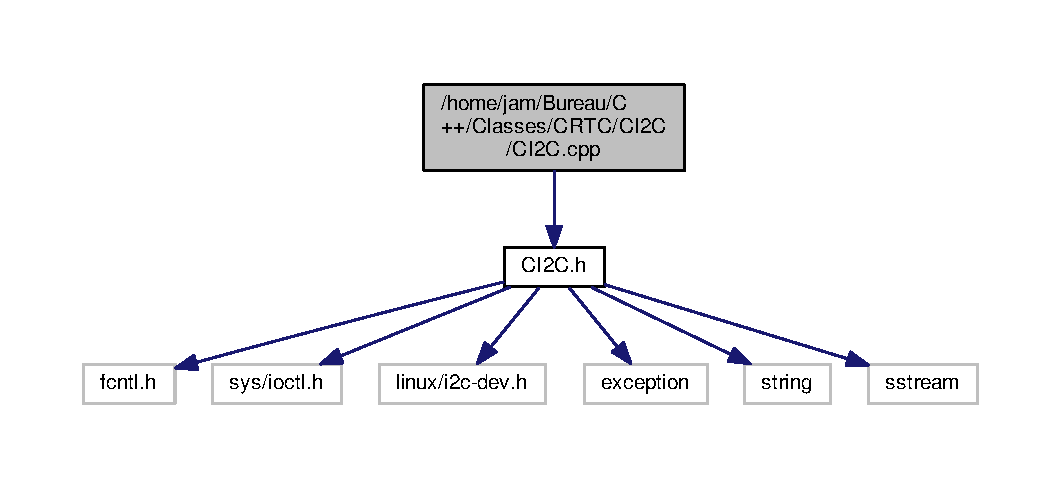
\includegraphics[width=350pt]{CI2C_8cpp__incl}
\end{center}
\end{figure}


\subsection{Description détaillée}
Contient la définition de la classe \hyperlink{classCI2C}{C\+I2\+C}. 

